
\section{Zasady działania kompasu (Zofia Sosińska)}\label{chap:naw}

Projekt kompasu jest na tyle prosty, aby nie przytłoczyć gracza nadmierną liczbą bodźców. Składa się z horyzontalnego, jednolitego paska,
 na którym wyświetlane są najważniejsze informacje o otoczeniu, symbol ośmiokąta, wskazujący na przestrzeń znajdującą się centralnie przed bohaterem
  oraz z bocznych pasków, wyróżniających końce narzędzia.

\begin{figure}[htbp]
    \centering
    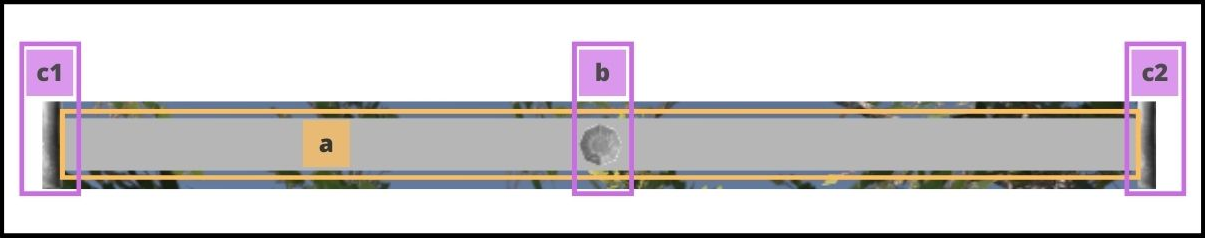
\includegraphics[width=0.9\textwidth]{images/ui/opis_ekementow_kompasu.png}
    \caption{Rozpiska elementów: a. główny pasek, b. symbol środka, c1., c2. paski końców kompasu.}\label{fig:compass_design}
\end{figure}
\FloatBarrier
Ikony wyświetlane na kompasie przedstawiają najważniejsze informacje w polu widzenia gracza, czyli stronę świata, w kierunku której jest on zwrócony, oraz przeciwników.
Poniżej przedstawiono kod odpowiedzialny za wyznaczenie pozycji symbolu na omawianym narzędziu. Wejściem jest komponent \texttt{RectTransform} symbolu przypisanego
danemu obiektowi oraz jego położenie. Po obliczeniu wektora prowadzącego do uzyskania np. pozycji wroga, wyznaczany jest kąt, o jaki musi się obrócić.
To jest przeliczane na pozycję na kompasie i jeśli obiekt znajduje się w polu widzenia postaci gracza to jest wyświetlany odpowiedni symbol.

\begin{figure}[htbp]
    \centering
    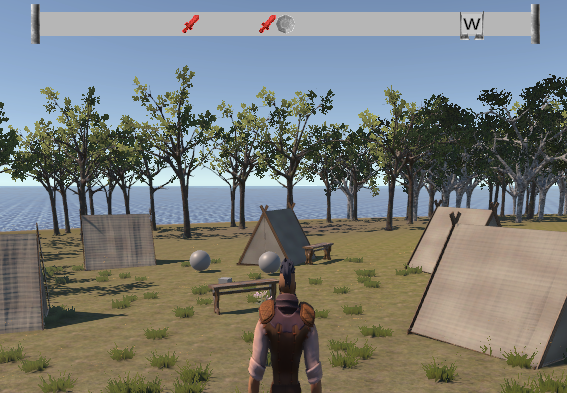
\includegraphics[width=0.9\textwidth]{images/ui/compass.png}
    \caption{Wizualizacja przypadku, w którym gracz patrzy centralnie na obozowisko wrogów. Na przeciwko oraz po lewej stronie znajdują się przeciwnicy, co jest zasygnalizowane na kompasie za pomocą symboli mieczy. Znajduje się na nim także informacja, że bohater jest lekko odchylony od Wschodu.
    }\label{fig:compass}
\end{figure}
\FloatBarrier
    \begin{lstlisting}[language=C++, caption=Fragment kodu odpowiedzialny za ustawienie symbolu na pasku kompasu.]
    void SetMarkerPosition(RectTransform markerTransform, Vector3 worldPosition)
    {
        Vector3 dirToTarget = worldPosition - CameraTransform.position;
        float angle = Vector2.SignedAngle(new Vector2(dirToTarget.x, dirToTarget.z), 
                                            new Vector2(CameraTransform.transform.forward.x, CameraTransform.transform.forward.z));
        float compassPositionX = Mathf.Clamp(
                                            2 * angle / Camera.main.fieldOfView, -1, 1);
        if (compassPositionX == 1 || compassPositionX == (-1))
        {
            markerTransform.anchoredPosition = new Vector2(0, 100);
        }
        else
        {
            markerTransform.anchoredPosition = new Vector2(
                compassBarTransform.rect.width / 2 * compassPositionX, 0);
        }
    }
    \end{lstlisting}
\FloatBarrier
Problem lokalizacji stron świata pojawił się, gdy nieprawidłowo wyświetlały się symbole po użyciu najprostszego rozwiązania. Na przykład dla Północy było to
pobranie wartości od \texttt{Vector3.forward}, co jest skrótowym zapisem \texttt{Vector3(0, 0, 1)}. Lewy dolny róg mapy jest położony w punkcie (0, 0, 0), co oznacza, że wymagane
jest przesunięcie, aby prawidłowo zasymulować strony świata. Północ i Południe  zostały przesunięte do połowy szerokości, a Wschód i Zachód - długości mapy. Każde z nich
zostało oddalone o 60000 jednostek, co pozwala na wiarygodną symulację stron świata na kompasie.

\begin{figure}[htbp]
    \centering
    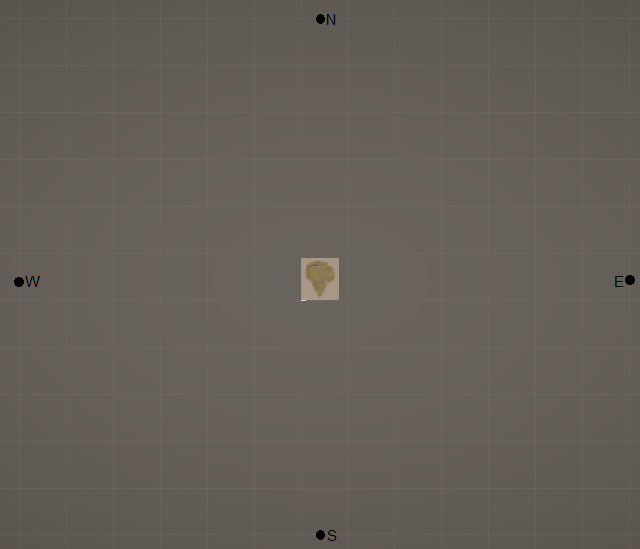
\includegraphics[width=0.9\textwidth]{images/ui/strony_swiata.png}
    \caption{Rozmieszczenie zasymulowanych stron świata.}\label{fig:world_sides}
\end{figure}
\FloatBarrier
Wykrycie wrogich jednostek znajduje się w funkcji Start. Każdemu obiektowi jest przypisywany symbol czerwonego miecza i w zależności od położenia wroga, obrazek wyświetlany jest odpowiednio na kompasie.
\begin{lstlisting}[language=C++, caption=Fragment kodu odpowiedzialny za połączenie wrogich obiektów na mapie z symbolami wyświetlonymi na kompasie]
    void SetPositionOfEnemies()
    {
        foreach (
            var e in enemiesOnMap.Zip(enemiesOnUI, (x, y) => new {enemyOnMap = x, 
                                                                    enemyOnUI = y }))
        {
            SetMarkerPosition(e.enemyOnUI.GetComponent<RectTransform>(), 
                                e.enemyOnMap.transform.position);
        }
    }
\end{lstlisting}
